\chapter{\label{ch:4-accel}Dependence Graph Model for FMU Co-simulation} 

\minitoc

This chapter describes a dependence graph model that is used in this thesis for representing a co-simulation program. The different phases for building such model are explained including the initial construction of the dependence graph, transformations that it undergoes in order to represent multi-rate co-simulation and mutual exclusion constraints, and finally rules for characterizing the graph with real-time parameters.
 
\section{\label{sec:4-depgrph}Dependence Graph of an FMU Co-simulation}

Automatic parallelization of computer programs embodies the adaptation of the potential parallelism inherent in the program to the effective parallelism that is provided by the hardware. Because computer programs are usually complex, this process of adaptation requires the use of a model for abstracting the program to be parallelized. The aim of using such model is to identify which parts of the program can be executed in parallel. The model has also to represent other features of the program such as data dependence between different pieces of the code. Task dependence graphs are commonly used for this purpose. A task dependence graph is a DAG denoted $G(V,A)$ where:
\begin{itemize}
\item $V$ is the set of vertices of the graph. The size of the graph $n$ is equal to the number of its vertices. Each vertex $v_i: 0 \leq i < n$ represents a task which is an atomic unit of computation.
\item $A$ is the set of arcs of the graph. A directed arc is denoted as a pair $(v_i,v_j)$ and describes a precedence constraint between $v_i$ and $v_j$, i.e. $v_i$ has to finish its execution before $v_j$ can start its execution. $v_i$ is called the \textit{tail} vertex and $v_j$ is called the \textit{head} vertex. 
\end{itemize}

The task dependence graph defines the partial order to be respected when executing the set of tasks. This partial order describes the potential parallelism of the program. %Figure \ref{} shows an example of a task dependence graph of size $5$.

The co-simulation of FMUs lends itself to the task dependence graph representation as shown hereafter. According to the FMI standard, the code of an FMU can be exported in the form of source code or as precompiled binaries. However, most FMU providers tend to adopt the latter option for proprietary reasons. We are thus interested in this case. The method for automatic parallelization of FMU co-simulation that we propose in this thesis is based on representing the co-simulation as a task dependence graph. We present in the rest of this section how this graph is constructed and a set of attributes that characterize it. The graph construction and characterization method is part of the RCOSIM approach as presented in \cite{benkhaled:2014}.

\subsection{Construction of the Dependence Graph of an FMU Co-Simulation}

The entry point for the construction of a task dependence graph of an FMU co-simulation is a user-specified set of interconnected FMUs as depicted in Figure~\ref{fig:2mdlsbb}. The execution of each FMU is seen as computing a set of input operations (one operation for each of the inputs of the FMU), a set of output operations (one operation for each of the outputs of the FMU), and one state operation for updating the state variables of the FMU. An operation is defined by a number of FMU C function calls. An input (resp. output ) operation is executed by calling \textit{fmiSet} (resp. \textit{fmiGet}) function and a state operation is executed by calling \textit{SetTime, GetDerivatives, SetContinuousStates, etc.}, functions in the case of FMI for Model Exchange or \textit{DoStep} function in the case of FMI for Co-Simulation. Thanks to FMI, it is additionally possible to access information about the internal structure of a model encapsulated in an FMU. In particular, as shown in Figure~\ref{fig:2mdlsintra}, FMI allows the identification of Direct Feedthrough (e.g. $Y_{B1}$) and Non Direct Feedthrough (e.g. $Y_{A1}$) outputs of an FMU and other information depending on the version of the standard:

\begin{itemize}
\item FMI 1.0: Dependence between input operations and output operations are given. The computation of the state at a given simulation step $k$ is considered necessary for the computation of each one of the output operations at the same simulation step $k$. It is considered that the computation of the state at a simulation step $k+1$ requires the computation of each of the input operations at the simulation step $k$.
\item FMI 2.0: In addition to the information provided in FMI 1.0, more information is given about data dependence. It is specified which output operations at a given simulation step depend on the state computation at the same step. Also, it is specified which input operations at a simulation step $k$ need to be computed before the computation of the state at the step $k+1$.  
\end{itemize}

\begin{figure}[htb]
\centering
\begin{subfigure}{.5\textwidth}
  \centering
  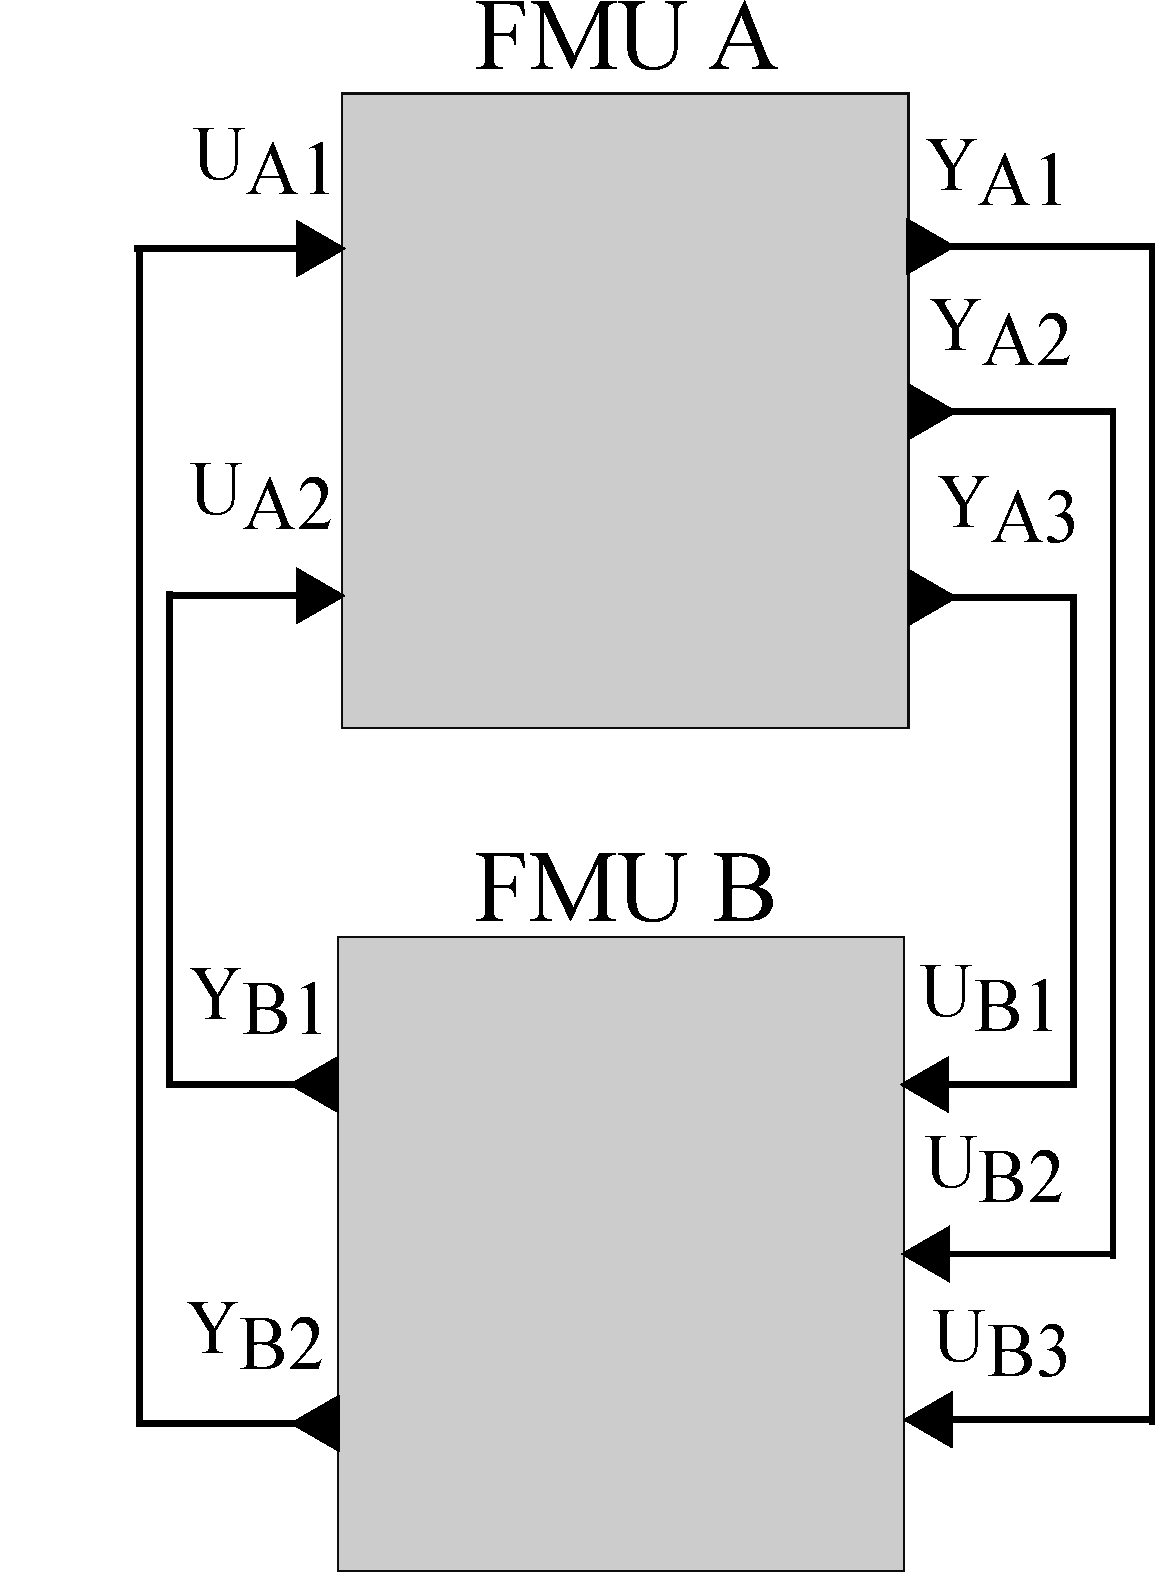
\includegraphics[scale=0.2]{figures/Two_Models_Black_Box}
  \caption{Inter-FMU dependence specified by the user}
  \label{fig:2mdlsbb}
\end{subfigure}%
\begin{subfigure}{.5\textwidth}
  \centering
  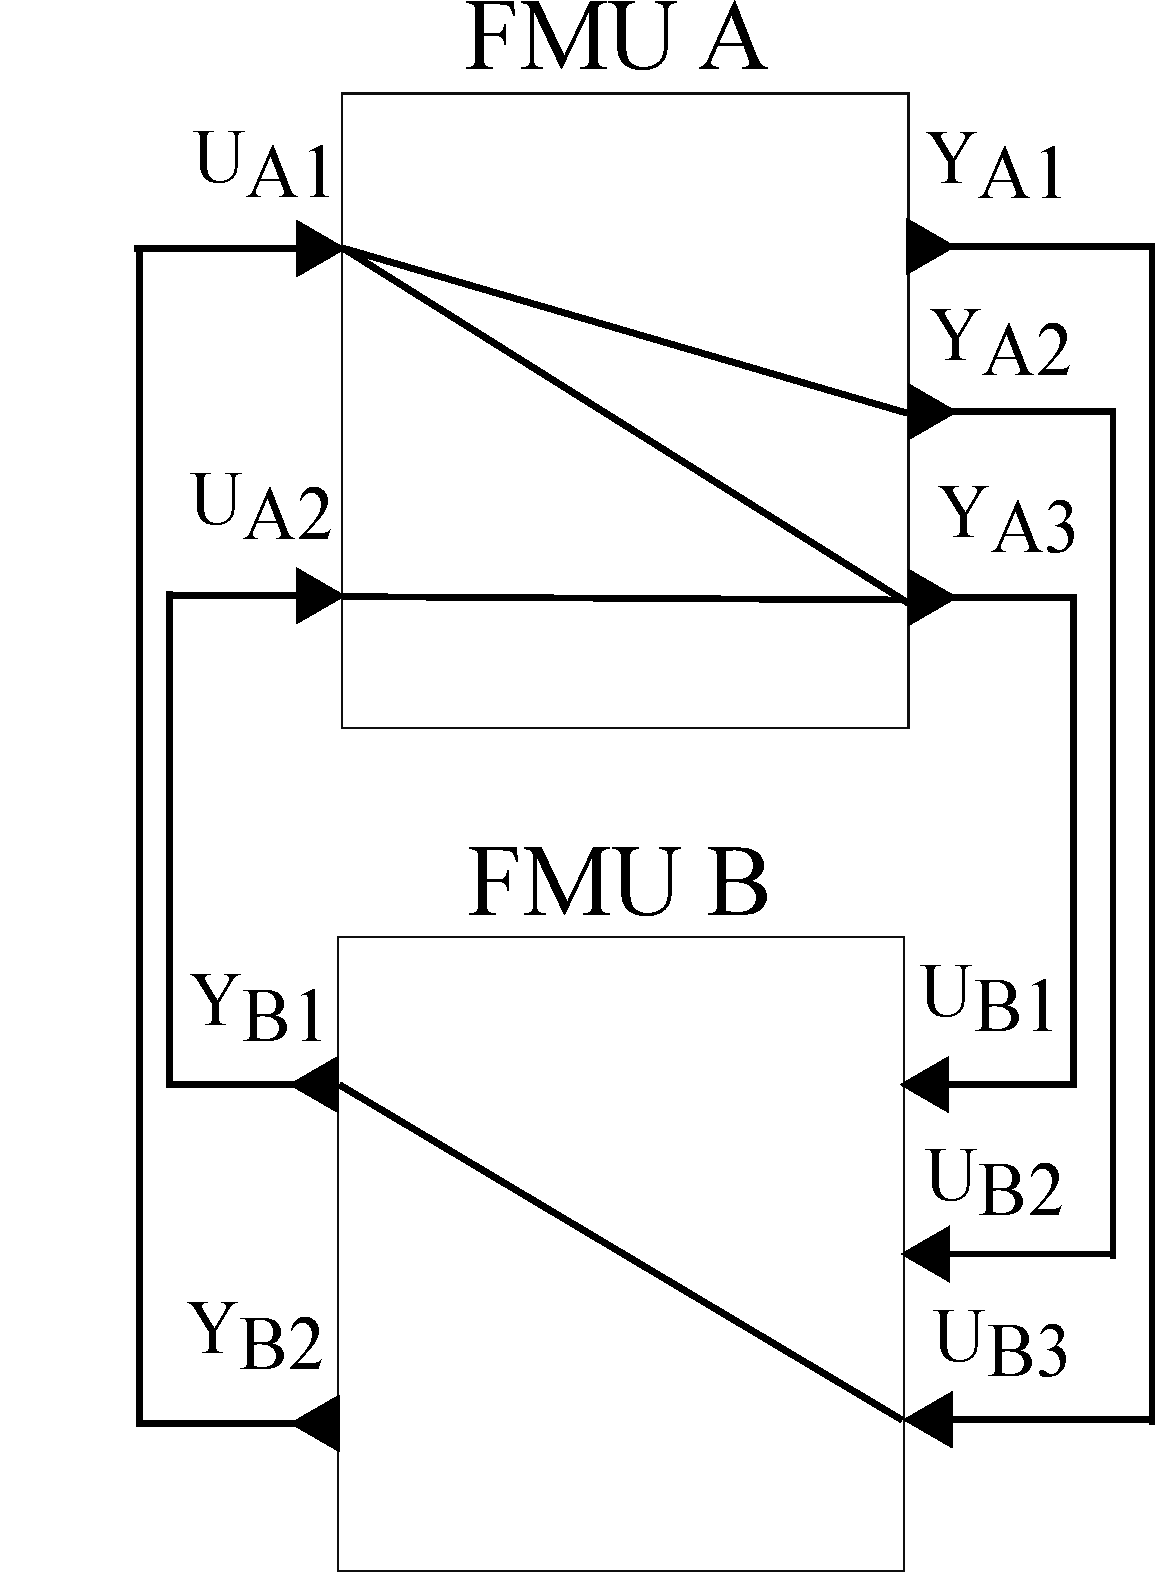
\includegraphics[scale=0.2]{figures/Two_Models}
  \caption{Intra-FMU dependence provided by FMI}
  \label{fig:2mdlsintra}
\end{subfigure}
\caption{An example of inter and intra-FMU dependence of two FMUs connected by the user}
\label{fig:2mdls}
\end{figure}

FMU information on input/output dependence allows building a graph with an increased granularity. The co-simulation is described by a task dependence graph $G(V,A)$ called the operation dependence graph where each vertex $o_i \in V: 0 \leq i < n$ represents one operation, each arc $(o_i,o_j) \in A: 0 \leq i,j < n$ represents a precedence relation between operations $o_i$ and $o_j$, and $n = |V|$ is the size of the operation dependence graph. The operation dependence graph is built by exploring the relations between the FMUs and between the operations of the same FMU. A vertex is created for each operation and arcs are then added between vertices if a precedence dependence exists between the corresponding operations. If FMI 1.0, which does not give information about the dependence between the state variables computation and the input and output variables computations, is used, we must add arcs between all input operations and the state operation of the same FMU. Furthermore, arcs connect all output operations and the state operation of the same FMU because the computation at the simulation step $k$ of an output must be performed with the same value of the state (computed at simulation step $k$) as for all the outputs belonging to the same FMU. Running the co-simulation consists in repeatedly executing the graph obtained that way. A new execution of the graph cannot be started unless the previous one was totally finished. The operation dependence graph corresponding to the FMUs of Figure~\ref{fig:2mdls} is shown in Figure~\ref{fig:dag}.

\begin{figure}[htb]
\centering
  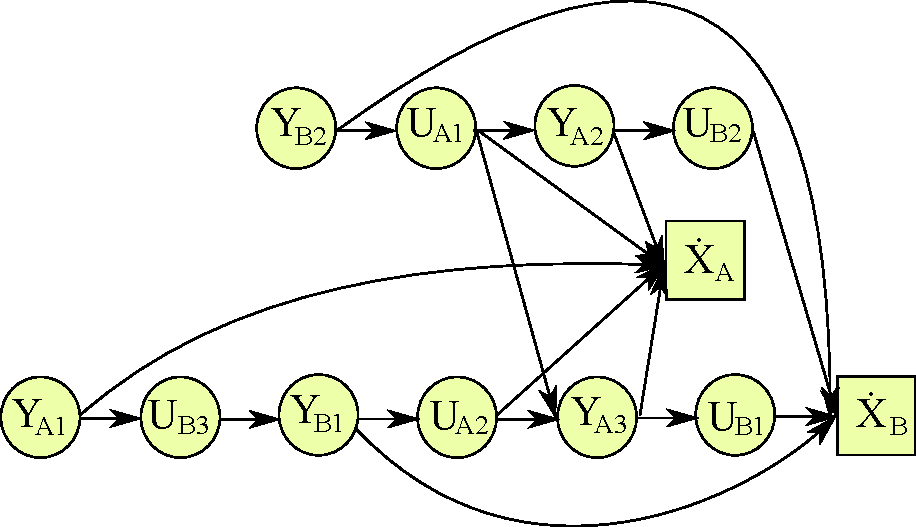
\includegraphics[scale=0.5]{figures/Operation_Graph_Two_Models}
\caption{Operation dependence graph obtained from the FMUs of Figure~\ref{fig:2mdls}}
\label{fig:dag}
\end{figure} 

\subsection{Dependence Graph Attributes}

In the remainder of the thesis, we shall use the term operation graph instead of operation dependence graph. The operation graph is used as input to the scheduling algorithm. In addition to the structure of the graph, the scheduling algorithm uses a number of attributes to compute an efficient schedule of the operation graph. Many list scheduling algorithms use attributes that are computed by the Critical Path Method \cite{}. We define a set of attributes and notations to characterize the operation graph.

The notation $f_m(o_i)$ is used to refer to the FMU to which the operation $o_i$ belongs, and $T(o_i)$ to denote the type of the operation $o_i$, i.e. $T(o_i) \in \{update_{input}, update_{output}, update_{state}\}$. $o_j$ is a predecessor of $o_i$ if there is an arc from $o_j$ to $o_i$, i.e. $(o_j, o_i) \in A$. We denote the set of predecessors of $o_i$ by $pred(o_i)$. $o_j$ is an ancestor of $o_i$ if there is a path in $G$ from $o_j$ to $o_i$. The set of ancestors of $o_i$ is denoted by $ance(o_i)$. $o_j$ is a successor of $o_i$ if there is an arc from $o_i$ to $o_j$, i.e. $(o_i, o_j) \in A$. We denote the set of successors of $o_i$ by $succ(o_i)$. $o_j$ is a descendant of $o_i$ if there is a path in $G$ from $o_i$ to $o_j$. The set of descendants of $o_i$ is denoted by $desc(o_i)$. A profiling phase allows measuring the execution time $C(o_i)$. For each operation, the average execution time of multiple co-simulation runs is used. When real-time execution is aimed, Worst Case Execution Times (WCET) are used instead. An operation $o_i$ is characterized by its communication step $H(o_i)$ which is equal to the communication step of its FMU. The earliest start time from start $S(o_i)$ and the earliest end time form start $E(o_i)$ are defined by equations \ref{eq:sfs} and \ref{eq:efs} respectively. $S(o_i)$ defines the earliest time at which the operation $o_i$ can start its execution. $S(o_i)$ is constrained by the precedence relations. The earliest time the operation $o_i$ can finish its execution is defined by $E(o_i)$.

\begin{equation}
S(o_i)=\begin{cases}
    0, & \text{if $pred(o_i)=\emptyset$}.\\
    max_{o_j \in pred(o_i)}(E(o_j)), & \text{otherwise}.
  \end{cases}
	\label{eq:sfs}
\end{equation}

\begin{equation}
	E(o_i)=S(o_i)+C(o_i) 
	\label{eq:efs}
\end{equation}

The latest end time from end denoted by $\overline{E}(o_i)$ and the latest start time from end denoted by $\overline{S}(o_i)$ are defined by equations \ref{eq:efe} and \ref{eq:sfe} respectively. %$\overline{E}(o_i)$ defines the latest time by which the operation $o_i$ must finish its execution so as not to increase the total execution time of the graph. For $o_i$ to finish its execution no later than $\overline{E}(o_i)$, it has to start its execution at the latest at $\overline{S}(o_i)$. 

\begin{equation}
\overline{E}(o_i)=\begin{cases}
    0, & \text{if $succ(o_i)=\emptyset$}.\\
    max_{o_j \in succ(o_i)}(\overline{S}(o_j)), & \text{otherwise}.
  \end{cases}
	\label{eq:efe}
\end{equation}

\begin{equation}
	\overline{S}(o_i)=\overline{E}(o_i)+C(o_i) 
	\label{eq:sfe}
\end{equation}

The critical path of the graph is the longest path in the graph. The length of a path is computed by accumulating the execution times of the operations that belong to it. The length of the critical path of the operation graph denoted by $R$ is defined by equation \ref{eq:crit}. The critical path is a very important characteristic of the operation graph. It defines a lower bound on the execution time of the graph, i.e. in the best case the time needed to execute the whole graph is equal to the length of the critical path. 

\begin{equation}
	R = \max_{o_i \in V_I}(E(o_i)) 
	\label{eq:crit}
\end{equation}
 
The flexibility $F(o_i)$ is defined by equation \ref{eq:flex}. $F(o_i)$ expresses the length of an execution interval within which operation $o_i$ can be executed without increasing the total execution time of the graph.

\begin{equation}
	F(o_i) = R - S(o_i) - C(o_i) - \overline{E}(o_i) 
	\label{eq:flex}
\end{equation}

\section{Dependence Graph of a Multi-rate FMU Co-simulation}

The operation graph model presented in the previous sections allows elementary modeling of FMU co-simulation programs. For some applications this model is sufficient to be used for multi-core scheduling. However, many industrial co-simulation applications feature behaviors that cannot be captured by this model. In particular, many industrial applications involve FMUs that are executed according to different communication steps. This is especially true when different FMUs of a co-simulation are provided by different parties. It is very common that an FMU provider designs the FMU in such a way that its proper functioning depends on the use of specific values of the communication step. It is therefore highly unrecommended, and in some cases even impossible, to change the communication step of the FMU. In other cases, even if it is possible and acceptable to change the communication step of a given FMU, better performance and/or accuracy could be obtained when using specific communication steps. As a consequence, our operation graph model has to be extended in order to accommodate multi-rate data exchange between operations. 

Consider an operation graph that is constructed as described in the previous section from a multi-rate co-simulation, i.e. some FMUs have different communication steps. Such graph is referred to as a multi-rate operation graph. One way for making such operation graph suitable for multi-core scheduling is to transform it into a mono-rate graph. This section presents an algorithm that transforms the initial multi-rate operation operation graph $G(V,A)$ into a mono-rate operation operation graph $G_M(V_M,A_M)$. The aim of this transformation is to ensure that each operation is executed according to the communication step of its respective FMU and also to maintain a correct data exchange between the different FMUs, whether they have different or identical communication steps. Similar algorithms have been used in the real-time scheduling literature \cite{kermia:2009, ramamritham:1995}.

We define the \textit{Hyper-Step (HS)} as the least common multiple ($lcm$) of the communication steps of all the operations: $HS=lcm(H(o_1),H(o_2), \dots ,H(o_n))$ where $n = |V_I|$ is the number of operations in the initial graph. The Hyper-Step is the smallest interval of time for describing a repeatable pattern of all the operations. The transformation algorithm consists first of all in repeating each operation $o_i$, $r_i$ times where $r_i$ is called the repetition factor of $o_i$ and $r_i = \frac{HS}{H(o_i)}$. Each repetition of the operation $o_i$ is called an occurrence of $o_i$ and corresponds to the execution of $o_i$ at a certain simulation step. We use a superscript to denote the number of each occurrence, for instance $o_i^s$ denotes the $s^{th}$ occurrence of $o_i$. Operations belonging to the same FMU have the same repetition factor since they are all executed according to the communication step of the FMU they belong to. Therefore, we define the repetition factor of an FMU to be equal to the repetition factor of its operations. Then, arcs are added between operations following the rules presented hereafter. Consider two operations $o_i, o_j \in V_I$ connected by an arc $(o_i,o_j) \in A_I$, then adding an arc $(o_i^s,o_j^u)$ to $A_M$, depends on the simulation steps (time) at which $o_i^s$ and $o_j^u$ are executed. In other words, if $k_{s}$ and $k_{u}$ are the simulation steps associated with $o_i^s$ and $o_j^u$ respectively, then the inequality $k_{s} \leq k_{u}$ is a necessary condition to add the arc $(o_i^s,o_j^u)$ to $A_M$. In addition, $o_j^u$ is connected with the latest occurrence of $o_i$ that satisfies this condition, i.e. with the occurrence $o_i^s$ such that $s=\max(0,1, \dots ,r_i-1) : k_{s} \leq k_{u}$. In the case where $H(o_i) = H(o_j)$ (and therefore $r_i = r_j$), occurrences $o_i^s$ and $o_j^u$ which correspond to the same number, i.e. $s = u$, are connected by an arc. On the other hand, if $H(o_i) \neq H(o_j)$, we distinguish between two types of dependence: we call the arc $(o_i,o_j) \in A_I$ a \textit{slow to fast} (resp. \textit{fast to slow}) dependence if $H(o_i) > H(o_j)$ (resp. $H(o_i) < H(o_j)$). For a slow to fast dependence $(o_i,o_j) \in A_I$, one occurrence of $o_i$ is executed while several occurrences of $o_j$ are executed. In this case, arcs are added between each occurrence $o_i^s: s \in \{0,1, \dots ,r_i-1\}$, and the occurrence $o_j^u$ such that:

\begin{equation}
u = \left \lceil{s \times \frac{H(o_i)}{H(o_j)}}\right \rceil\;
\end{equation}

We recall that for a slow to fast dependence, the master algorithm can preform extrapolation of the inputs of the receiving FMU. For a fast to slow dependence $(o_i,o_j) \in A_I$, arcs are added between each occurrence $o_i^s$, and the occurrence $o_j^u: u \in \{0,1, \dots ,r_j-1\}$ such that:

\begin{equation}
s = \left \lfloor{u \times \frac{H(o_j)}{H(o_i)}}\right \rfloor\;
\end{equation}

Arcs are added also between the occurrences of the same operation, i.e. $(o_i^s,o_i^{s'})$ where $s \in \{0,1, \dots ,r_i-2\}$ and $s' = s + 1$. Finally, for each FMU, arcs are added between the $s^{th}$ occurrence of the state operation, where $s \in \{0,1, \dots ,r_i-2\}$, and the $(s+1)^{th}$ occurrences of the input and output operations. The multi-rate graph transformation is detailed in Algorithm \ref{algo:mr}. The algorithm traverses all the graph by applying the aforementioned rules in order to transform the graph and finally stops when all the nodes and the edges have been visited.

\begin{algorithm}[htb]
		%Initialization\;
		\textbf{Input:} Initial operation operation graph $G_I(V_I,A_I)$\; 
		\textbf{Output:} Transformed operation operation graph $G_M(V_M,A_M)$\;
		Set $G_I(V_I,A_I)$ the initial multi-rate operation operation graph and $G_M(V_M,A_M)$ the new mono-rate graph\; 
		$V_M \leftarrow \emptyset$; $A_M \leftarrow \emptyset$\;
		\ForEach{operation $o_i \in V_I$}
		{
			Compute the repetition factor of $o_i$: $r_i \leftarrow \frac{HS}{H(o_i)}$\;
			Repeat the operation $o_i$: $V_M \leftarrow V_M \cup \{o_i^s\}, s \in \{0, \dots,r_i-1\}$\;
		}
		\ForEach{arc $(o_i,o_j) \in A_I$}
		{
			\If{$H(o_i) > H(o_j)$ ($(o_i,o_j)$ is a slow to fast dependence)}
			{
					Compute $u = \left \lceil{s \times \frac{H(o_i)}{H(o_j)}}\right \rceil$ and add the arc $(o_i^s,o_j^u)$ to the new graph $G_M(V_M,A_M)$: $A_M \leftarrow A_M \cup \{(o_i^s,o_j^u)\}, s \in \{0, \dots,r_i-1\}$\;
				
			}
			\ElseIf{$H(o_i) < H(o_j)$ ($(o_i,o_j)$ is a fast to slow dependence)}
			{
				
					Compute $s = \left \lfloor{u \times \frac{H(o_i)}{H(o_j)}}\right \rfloor$ and add the arc $(o_i^s,o_j^u)$ to the new graph $G_M(V_M,A_M)$: $A_M \leftarrow A_M \cup \{(o_i^s,o_j^u)\}, u \in \{0, \dots,r_j-1\}$\;
				
			}
			\Else
			{
				
					Add the arc $(o_i^s,o_j^s)$ to the new graph $G_M(V_M,A_M)$: $A_M \leftarrow A_M \cup \{(o_i^s,o_j^s)\}, s \in \{0, \dots,r_i-1\}$\;
				
			}
		}
		\ForEach{operation $o_i \in V$}
		{
			
				Add an arc between successive occurrences of $o_i$: $A_M \leftarrow A_M \cup \{(o_i^s,o_i^{s+1})\}, s \in \{0, \dots,r_i-2\}$\;
			
		}
		\ForEach{operation $o_i \in V$ such that $T(o_i) = state$}
		{
					Add arcs $(o_i^s,o_j^{s+1})$ to the new graph $G_M(V_M,A_M)$ between $o_i$ and every operation $o_j$ such that $M(o_j)=M(o_i)$ and $T(o_j) \in \{input,output\}$: $A_M \leftarrow A_M \cup \{(o_i^s,o_j^{s+1})\}, s \in \{0, \dots,r_i-2\}$\;
				
		}
	\caption{Multi-rate graph transformation algorithm}
	\label{algo:mr}
\end{algorithm}

Figure \ref{fig:dagmr} shows the graph obtained by applying the multi-rate transformation algorithm on the graph of Figure \ref{fig:dag}. In this example $H_B = 2 \times H_A$, where $H_A$ and $H_B$ are the communication steps of FMUs $A$ and $B$ respectively.

\begin{figure}[htb]
\centering
  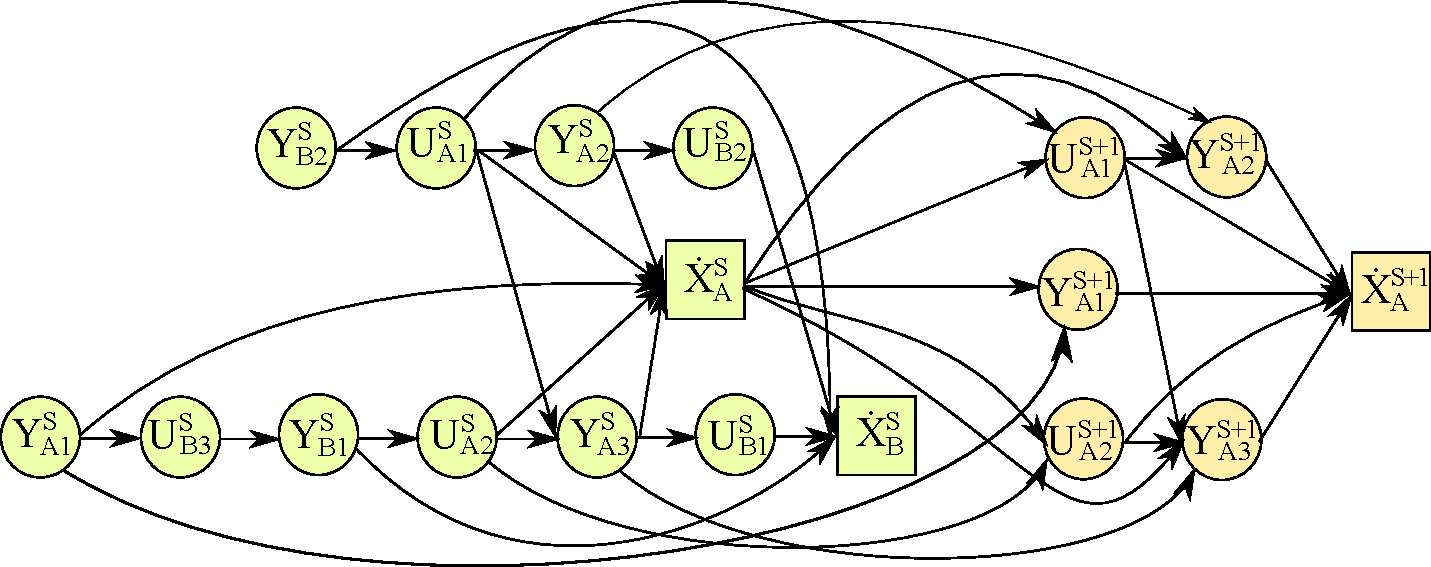
\includegraphics[scale=0.5]{figures/Operation_Graph_Two_Models_Multirate}
\caption{Graph obtained by applying the multi-rate transformation algorithm on the graph of Figure~\ref{fig:dag}}
\label{fig:dagmr}
\end{figure}

Without loss of generality, the superscript which denotes the number of the occurrence of an operation is not used in the remainder of the thesis for the sake of clarity. Each vertex of the graph $G(V,A)$ represents an operation that is referred to using the notation $o_i$.

\section{Dependence Graph with Mutual Exclusion Constraints}
The FMI standard states that \textit{``FMI functions of one instance don't need to be thread safe''}. Therefore, an FMU does not implement any service to support concurrent access to its functions from multiple threads, and it is up to the executing environment to ensure the calling sequences of functions are respected as specified in the FMI standard. These restrictions introduce mutual exclusion constraints on the operations of the same FMU. We propose in this section an offline method for lightweight handling of these constraints.

\subsection{Motivation}

In order to study the impact of mutual exclusion constraints, we have evaluated the performance obtained using two mutual exclusion strategies. The first one uses a dedicated lock (system object that guarantees mutual exclusion) for each FMU: every time an FMU function call is made at runtime, the associated lock has to be acquired before the execution of the function code can be started. The second solution is explained in \cite{benkhaled:2014} and consists in allocating the operations of a same FMU to the same core (constrained allocation). The scheduling heuristic that was used in these tests is presented in chapter \ref{ch:5-sched}. The theoretical speed-up was estimated by computing the makespan of the graph. Results are given in Figure \ref{fig:theoretical-speedup}. It shows that the expected speed-up in the case of constrained allocation is less than the one using unconstrained allocation, when the number of cores is less than five, but similar when five cores or more are available. When using less than five cores, the large number of $update_{output}$ operations can be efficiently allocated only if the unconstrained allocation is used: the speed-up difference between the constrained and unconstrained allocation cases is due to this restriction on the allocation. Five is the minimal number of cores for enabling the execution of each $update_{state}$ operation on a different core. Due to the predominant execution times of the $update_{state}$ operations, their impact on the speed-up overrides the possibility of optimizing the allocation of the other operations. This explains why the speed-up difference between the unconstrained and the constrained allocation cases becomes very small with five cores or more.

\begin{figure}[phbt]
\centering
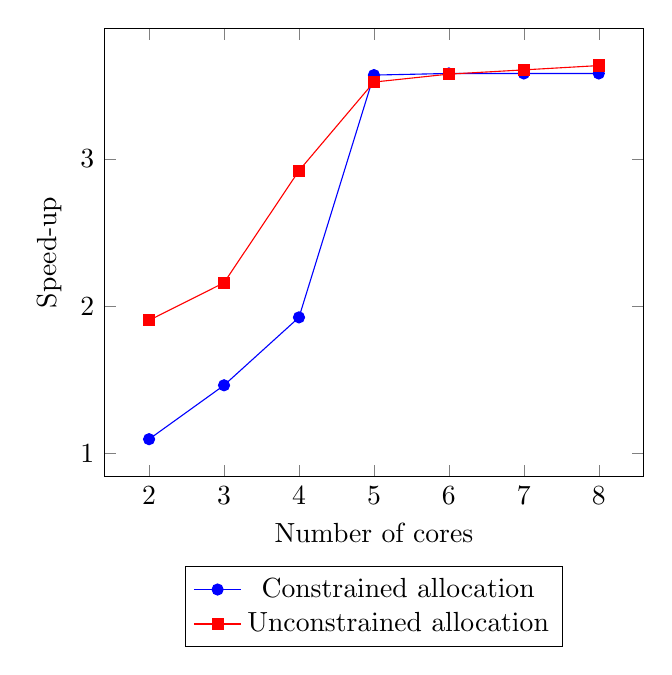
\begin{tikzpicture}
    \begin{axis}[
        xlabel=Number of cores,
        ylabel=Speed-up,legend style={at={(0.5,-0.2)},anchor=north}]
    \addplot[mark=*,blue,label=const] plot coordinates {
        (2,     1.097909998)
        (3,    1.463604418)
        (4,    1.924422442)
        (5,   3.568543452)
        (6,   3.579496624)
        (7,   3.579496624)
        (8,  3.579496624)
    };
    \addlegendentry{Constrained allocation}

    \addplot[color=red,mark=square*,label=unconst]
        plot coordinates {
        (2,     1.904310908)
        (3,    2.15962963)
        (4,   2.91987982)
        (5,   3.521135266)
        (6,  3.575107296)
        (7,  3.603831891)
        (8,  3.633021807)
        }; 
    \addlegendentry{Unconstrained allocation}
    \end{axis}
\end{tikzpicture}
\caption{Theoretical speed-up.}
\label{fig:theoretical-speedup}
\end{figure}

We implemented and tested both mutual exclusion strategies in order to compare their runtime performance. Tests were performed using the industrial use case described in chapter \ref{ch:6-eval}. Execution times measurements were performed by getting the system time stamp at the beginning of the execution and after $30$ seconds of the simulated time. As previously, we compared the speed-up by dividing the mono-core co-simulation execution time by the co-simulation execution time on a fixed number of cores. Figure \ref{fig:real-speedup} sums up the results, where unconstrained allocation corresponds to the use of lock objects. It shows the impact of mutex overhead on the speed-up. Whatever the number of the available cores, the speed-up remains close to $1.3$. On the contrary, the implementation of the constrained allocation gives similar results in terms of speed-up improvement when increasing the number of cores until five. Nevertheless, the maximum measured speed-up ($2.4$) remains smaller than the theoretical one ($3.5$). In fact, the theoretical speed-up computation considers the makespan ratio without any estimation of the runtime overhead which certainly has an important impact on the speed-up.


\begin{figure}[phbt]
\centering
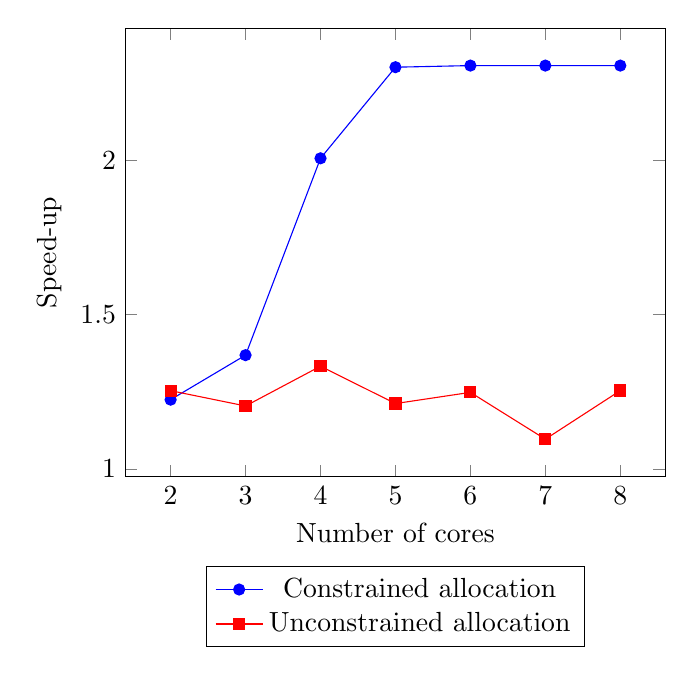
\begin{tikzpicture}
    \begin{axis}[
        xlabel=Number of cores,
        ylabel=Speed-up,legend style={at={(0.5,-0.2)},anchor=north}]
    \addplot[mark=*,blue,label=const] plot coordinates {
        (2,     1.223967163)
        (3,    1.368187328)
        (4,    2.005976773)
        (5,   2.301174325)
        (6,   2.306397786)
        (7,   2.306397786)
        (8,  2.306397786)
    };
    \addlegendentry{Constrained allocation}

    \addplot[color=red,mark=square*,label=unconst]
        plot coordinates {
        (2,     1.253126949)
        (3,    1.203511837)
        (4,   1.332430943)
        (5,   1.211351319)
        (6,  1.247650948)
        (7,  1.095957175)
        (8,  1.253420685)
        }; 
    \addlegendentry{Unconstrained allocation}
    \end{axis}
\end{tikzpicture}
\caption{Measured speed-up.}
\label{fig:real-speedup}
\end{figure}

%The obtained results show the importance of employing a mutual exclusion strategy that is efficient with regards to the limitations of allocating the operations and the introduced synchronization overhead. In the rest of this section, we attempt to attain this objective.

The restrictions introduced by employing the tested mutual exclusion techniques makes it highly desirable to find an alternative solution that could satisfy the mutual exclusion constraints while: \begin{inlinelist} \item leaving as much flexibility as possible for allocating the operations to the cores and; \item introducing lower synchronization overhead \end{inlinelist}. In the rest of this section, we suggest a method for offline handling of mutual exclusion constraints. The proposed method is based on modeling the mutual exclusion constraints in the operation graph of the co-simulation.

\subsection{Acyclic Orientation of Mixed Graphs}

The operation graph model can be extended in order to represent scheduling problems that involve precedence constraints and mutual exclusion constraints. This is commonly done using \textit{mixed graphs}. A mixed graph $G(V,A,D)$ is a graph which contains a set $A$ of directed arcs denoted $(o_i,o_j): 0 \leq i, j < n$ and a set $D$ of undirected edges denoted $[o_i,o_j]: 0 \leq i, j < n$. In the scheduling literature, these graphs are known also as disjunctive graphs. In addition to the precedence constraints represented by arcs as described in section \ref{sec:4-depgrph}, mutual exclusion relations are represented by edges in a mixed graph such that: 
\begin{itemize}
\item \textit{Precedence constraints:} $\forall (o_i,o_j) \in A, o_i$ must finish its execution before $o_j$ can start its execution.  
\item \textit{Mutual exclusion constraints:} $\forall [o_i,o_j] \in D, o_i$ and $o_j$ must be executed in strictly disjoint time intervals.
\end{itemize}

Operations belonging to the same FMU can be executed in either order but not in parallel. In order to compute a schedule for a mixed graph, an execution order has to be defined for each pair of operations connected by an edge which is interpreted by assigning a direction to this edge. Cycles must not be introduced in the graph while assigning directions to edges, otherwise, the scheduling problem becomes infeasible \cite{}. Since the final goal is to accelerate the execution of the co-simulation, and in other words, minimize the makespan of the execution of the operation graph, the acyclic orientation of the mixed graph has to minimize the length of the critical path of the graph.

%\subsubsection{Graph Coloring of Undirected Graphs}
% Talk about Gallai–Hasse–Roy–Vitaver theorem
The acyclic orientation problem is closely related to vertex coloring. In its general form, i.e. when all edges of the graph are undirected, vertex coloring is a function $\alpha: V \rightarrow \{1, 2, \ldots, k\}$ which labels the vertices of the graph with integers, called colors, such that the inequality \ref{eq:color1} holds.

\begin{equation}
\forall\ [o_i,o_j] \in D,\ \alpha(o_i) \neq \alpha(o_j)
\label{eq:color1}
\end{equation}

The acyclic orientation of the graph can then be obtained by assigning a direction to every edge such that the color of the corresponding tail vertex is smaller than the color of the corresponding head vertex. A graph coloring with $k$ colors is referred to as \textit{k-coloring}. In its general form, vertex coloring aims at finding a \textit{minimum vertex coloring}, i.e. minimizing $k$ the number of the used colors. The minimum number of colors required to color an undirected graph is called the chromatic number and is denoted $\chi(G)$. The Gallai–Hasse–Roy–Vitaver theorem \cite{gallai:1968,roy:1967,hasse:1966,vitaver:1962} links the length of the longest path in orientations of the graph to vertex coloring of the graph. It states that the length of the longest path of a directed graph is at least $\chi(G)$. Thus, a minimum vertex coloring leads to an acyclic orientation that minimizes the length of the critical path of the resulting graph. Computing the chromatic number of a graph is NP-complete.

The acyclic orientation of a mixed graph can be obtained similarly. However, vertex coloring of a mixed graph has to take into account both arcs and edges of the graph. More precisely, a vertex coloring of a mixed graph is a function $\alpha: V \rightarrow \{1, 2, \ldots, k\}$ such that inequalities \ref{eq:color1} and \ref{eq:color2} hold.

\begin{equation}
\forall\ (o_i,o_j) \in A,\ \alpha(o_i) < \alpha(o_j)
\label{eq:color2}
\end{equation}

A coloring of a mixed graph $G(V,A,D)$ exists only if it is cycle-free \cite{ries:2007}, i.e. the directed graph $G(V,A,\emptyset)$ does not contain any cycle. The problem of acyclic orientation of mixed graphs has been studied in the literature in \cite{andreev:2000,sotskov:2002,al-anzi:2006}. Efficient algorithms have been proposed for special types of graphs, however in the general case it has been shown that the problem is NP-Hard.

\subsection{Problem Formulation}

Let $G(V,A)$ be a operation graph of an FMU co-simulation constructed as described in section \ref{sec:4-depgrph}. In order to represent mutual exclusion constraints between FMU operations, the initial operation graph $G(V,A)$ is transformed into a mixed graph by connecting each pair of mutually exclusive operations $o_i, o_j$ by and edge $[o_i, o_j]$. The resulting mixed graph is denoted $G(V,A,D)$, where $V$ is the set of operations, $A$ is the set of arcs, and $D$ is the set of edges. Once the mixed graph is constructed, directions have to be assigned to its edges in order define an order of execution for mutually exclusive operations. The timing constraints represented by the mixed graph $G(V,A,D)$ are given by expressions \ref{eq:color4} and \ref{eq:color5}. If operations $o_i$ and $o_j$ are connected by an arc $(o_i,o_j)$, the time interval $(S(o_i), E(o_i)]$ must precede the time interval $(S(o_j), E(o_j)]$. Otherwise, if operations $o_i$ and $o_j$ are connected by an edge $[o_i,o_j)]$, time intervals $(S(o_i), E(o_i)]$ and $(S(o_j), E(o_j)]$ must be strictly disjoint.

\begin{equation}
\forall\ (o_i,o_j) \in A,\ E(o_i) \leq S(o_j)
\label{eq:color4}
\end{equation}

\begin{equation}
\forall\ [o_i,o_j] \in D,\  (S(o_i), E(o_i)] \cap (S(o_j), E(o_j)] = \emptyset
\label{eq:color5}
\end{equation}

The timing attributes of the operations in the mixed graph $G(V,A,D)$ are the same as in the initial graph $G(V,A)$ because the added set of edges $[o_i, o_j] \in D$ does not impact the computation of these attributes. The attributes of an operation $o_i$, connected by an edge with another operation, may change only when this edge is assigned a direction. 

An edge $[o_i,o_j]$ is called a conflict edge if the intervals $(S(o_i), E(o_i)]$ and $(S(o_j), E(o_j)]$ as computed in the graph $G(V,A)$ overlap (equation \ref{eq:conflict}). If for a given edge $[o_i,o_j]$ either $E(o_i) \leq S(o_j)$ or $E(o_j) \leq S(o_i)$, there is no conflict and the edge can be assigned a direction. 

\begin{equation}
E(o_i) > S(o_j)\ \text{and}\ E(o_j) > S(o_i)
\label{eq:conflict}
\end{equation}

It should be noted that, for a given edge $[o_i, o_j]$, choosing either of the execution orders does not impact the numerical results of the co-simulation since these operations do not have data dependence. Still, we have to ensure mutual exclusion between them due to the non-thread-safe implementation of FMI. Following the definition given the previous section, the corresponding coloring is a function $\alpha: V \rightarrow \{1, 2, \ldots, k\}$ which is equivalent to mapping the operations $o_i \in V$ to the time intervals $[S(o_1), E(o_1)], [S(o_2), E(o_2)], \ldots, [S(o_n), E(o_n)]$.

The problem of acyclic orientation of the mixed graph $G(V,A,D)$ can be stated as an optimization formulation as follows:

\begin{itemize}[label={},topsep=1pt,parsep=1pt,partopsep=1pt,leftmargin=*]	
\item \textbf{Input:} Mixed graph $G(V,A,D)$
\item \textbf{Output:} DAG $G(V,A)$
\item \textbf{Find:} Coloring $\alpha: V \rightarrow \{1, 2, \ldots, k\}$
\item \textbf{Minimize:} Number of colors $k$
\item \begin{subjecto}
			      \item $\forall\ (o_i,o_j) \in A,\ \alpha(o_i) < \alpha(o_j)$
				   	\item $\forall\ [o_i,o_j] \in D,\ \alpha(o_i) \neq \alpha(o_j)$
       \end{subjecto}
\end{itemize}

This formulation is stated as a vertex coloring problem, however, it is possible to state the problem and its solution using either vertex coloring notation or the scheduling notation. Thus, we note the following equivalence:

\begin{itemize}[label={},topsep=1pt,parsep=1pt,partopsep=1pt,leftmargin=*]	
\item Coloring $\alpha: V \rightarrow \{1, 2, \ldots, k\} \equiv$ Mapping $\alpha: V \rightarrow \{[S(o_1), E(o_1)],$ $[S(o_2), E(o_2)],$ $\ldots,$ $[S(o_n), E(o_n)]\} \equiv$ Assignment $\alpha: D \rightarrow \{(o_i,o_j),(o_j,o_i): [o_i,o_j] \in D\}$
\item $\forall\ (o_i,o_j) \in A,\ \alpha(o_i) < \alpha(o_j) \equiv \forall\ (o_i,o_j) \in A,\ E(o_i) \leq S(o_j)$
\item $\forall\ [o_i,o_j] \in D,\ \alpha(o_i) \neq \alpha(o_j)$ $\equiv$ $\forall\ [o_i,o_j] \in D,\  (S(o_i), E(o_i)] \cap (S(o_j), E(o_j)] = \emptyset$
\item Optimal coloring $min(k)$ $\equiv$ Optimal length of the critical path $min(R)$
\end{itemize}

\subsection{Resolution using Integer Linear Programming}

Let $G(V,A,D)$ be a mixed graph constructed form the operation graph $G(V,A)$ as described in the previous sections to represent precedence and mutual exclusion constraints between operations of an FMU co-simulation. In the following, we present an Integer Linear Programming formulation for the problem of acyclic orientation of $G(V,A,D)$. The proposed formulation is based on the scheduling notation which gives a more compact set of constraints compared to a formulation that uses the vertex coloring notation.

\subsubsection{Variables and Constants}

Tables \ref{table:varilporient} and \ref{table:consilporient} summarize the variables and the constants that are used in the ILP formulation respectively.

\begin{table}[!htbp]
\caption{Variables used in the ILP formulation of the acyclic orientation problem}
\centering
\label{table:varilporient}
\begin{tabular}{l l l}
\toprule
Variable & Type & Description  \\
\midrule
 $S(o_i)$ & Integer & Start time of operation $o_i$\\
 $E(o_i)$ & Integer & End time of operation $o_i$\\
 $b_{ij}$ & Binary & Orientation decision variable associated with edge $[o_i,o_j] \in D$\\
 $P$ & Integer & Length of the critical path of the graph\\
\bottomrule
\end{tabular}
\end{table}

\begin{table}[!htbp]
\caption{Constants used in the ILP formulation of acyclic orientation problem}
\centering
\label{table:consilporient}
\begin{tabular}{l l l}
\toprule
Constant & Type & Decription\\
\midrule
 $C(o_i)$ & Integer & Execution time of operation $o_i$\\
 $M$ & Integer & Large positive number\\
\bottomrule
\end{tabular}
\end{table}

\subsubsection{Constraints}

The following set of constraints is used in the ILP formulation of the acyclic orientation problem:

\begin{itemize}

\item \textit{Precedence constraints:} The start time of each operation is equal to the maximum of the end times of all its predecessors. Expression \ref{orient:const_1} captures this constraint. Note that expression $orient:const_1$ indicates that the start time of operation $o_j$ if greater or equal to the end time of each predecessor $o_i$. This is sufficient to express $S(o_j) = max_{o_i \in pred(o_j)}(E(o_i))$ since the formulated problem is a minimization problem.

\begin{equation}
\forall (o_i,o_j) \in A, S(o_j) \geq E(o_i):
\label{orient:const_1}
\end{equation}

\item \textit{Mutual exclusion constraints:} We define the binary variable $b_{ij}$ which is associated with the direction that is assigned to edge $[o_i,o_j]$. $b_{ij}$ is set to $1$ if the edge $[o_i,o_j]$ is assigned a direction from $o_i$ to $o_j$, i.e. $\alpha([o_i,o_j]) = (o_i,o_j)$ and to $0$ otherwise. Note that $b_{ij}$ is the complement of $b_{ji}$. For every pair of operations that are connected by and edge, we have to ensure that their time intervals are strictly disjoint, i.e. $\forall\ [o_i,o_j] \in D,\  (S(o_i), E(o_i)] \cap (S(o_j), E(o_j)] = \emptyset$. Expressions \ref{orient:const_2} and \ref{orient:const_3} capture this constraint where $M$ is a large positive integer.

\begin{equation}
\forall [o_i,o_j] \in E, S(o_i) \geq E(o_j) - M \times (1-b_{ij})
\label{orient:const_2}
\end{equation} 

\begin{equation}
\forall [o_i,o_j] \in E, S(o_j) \geq E(o_i) - M \times b_{ij}
\label{orient:const_3}
\end{equation}

\item \textit{Time intervals:} Expression \ref{orient:const_4} is used to compute the end time of each operation.

\begin{equation}
\forall o_i \in V, E(o_i) = S(o_i) + C(o_i)
\label{orient:const_4}
\end{equation} 

\item \textit{Length of the critical path:} The critical path $P$ is equal to the maximum of the end times of all the operations (expression \ref{orient:const_5}).

\begin{equation}
\forall o_i \in V, P \geq E(o_i)
\label{orient:const_5}
\end{equation}

\end{itemize}

\subsubsection{Objective}

The objective of this linear program is to minimize the length of the critical path of the operation graph (expression \ref{orient:obj}).

\begin{equation}
min(P)
\label{orient:obj}
\end{equation}


\subsection{Acyclic Orientation Heuristic}

We propose in this section a heuristic for the acyclic orientation of the mixed graph $G(V,A,D)$. A straightforward acyclic orientation can be obtained by sorting the operations in a non decreasing order of their start times $S(o_i)$ and assigning directions to edges following this order, i.e. $\forall [o_i,o_j] \in D, S(o_i) \leq S(o_j), \alpha([o_i,o_j]) = (o_i,o_j)$. This a fast greedy acyclic orientation, however it can be improved as we will show hereafter.

Let $d$ be the sum of the repetition factors of all the FMUs. The set of operations $V$ can be represented as a union of mutually disjoint non empty subsets such that every subset contains all operations that belong to the same FMU and that correspond to the same occurrence:

\begin{equation}
V = \bigcup_{k=1}^d V_k, \forall\ o_i^p, o_j^q \in V_k, k \in \{0, 1, \ldots, d\}, f_m(o_i^p)=f_m(o_j^q)\ \text{and}\ p = q
\label{eq:opsubset}
\end{equation}

It is know that edges in the set $D$ exist only between operations that belong to the same FMU. Furthermore, for every edge $[o_i^p,o_j^q] \in D$, operations $o_i$ and $o_j$ correspond to the same occurrence. Even if operations which belong to the same FMU and correspond to different occurrences are mutually exclusive, it is not needed to connect them by an edge because an execution order is already ensured for these operations by the way the operation graph is constructed. In other words, all the operations of an FMU, and which correspond to the same occurrence have to finish their execution before the next occurrence of any operation can start its execution. Similarly to the operation set, the edge set $D$ can be subdivided into mutually disjoint non empty subsets:

\begin{equation}
D = \bigcup_{k=1}^d D_k, \forall\ [o_i^p, o_j^q] \in D_k, k \in \{0, 1, \ldots, d\}, f_m(o_i^p)=f_m(o_j^q)\ \text{and}\ p = q
\label{eq:opsubset}
\end{equation}

In view of the above, we define the set of subgraphs which constitute the graph $G(V,\emptyset,D) = \bigcup_{k=1}^d G(V_k,D_k)$. Lemma \ref{lemma:orient} indicates the relationship between the acyclic orientations of the subgraphs $G(V_k,D_k)$ and the acyclic orientation of the mixed graph $G(V,A,D)$.

\begin{lemma}
An acyclic orientation of the mixed graph $G(V,A,D)$ can be obtained by finding an acyclic orientation for every subgraph $G_k(V_k,D_k)$ following the non decreasing order of the start times of the operations as described previously.
\label{lemma:orient}
\end{lemma}

\begin{proof}
 In order to prove this, we have to show that every edge in $D$ is assigned a	direction and that the resulting orientation does not lead to the creation of a cycle. Since every edge $[o_i, o_j]$ belongs to one subset of edges $D_k$, finding acyclic orientations for all the subgraphs $G_k(V_k)$ leads to assigning a direction to every edge in $D$. The existence of a cycle in the resulting graph means that there exists at least an edge $[o_i,o_j]$ that has been transformed into the arc $(o_i,o_j)$ and $S(o_i) > S(o_j)$. However, this is not possible because the greedy acyclic orientation assigns directions to edges following a non-decreasing order of the start times of the operations.
\end{proof}

Consider now that the acyclic orientation of each subgraph $G_k(V_k,D_k)$ is obtained by finding a vertex coloring for this subgraph. This vertex coloring can be seen as a sequence of assignments $\alpha_1, \alpha_2, \ldots, \alpha_{|D_k|}$, such that every assignment $\alpha_l$ assigns a color to one operation $o_i \in V_k$ and leads to assigning directions to edges that connect $o_i$ with other already colored operations $o_j \in V_k$. The number of assignments needed to perform the acyclic orientation of $G_k(V_k,D_k)$ is equal to the number of edges $|D_k|$. Following the coloring of an operation and the engendered assignment of directions, the attributes of some operations may change. Two situations have to be distinguished:

\begin{itemize}
\item Coloring $\alpha_l$ of operation $o_i$ does not lead to assigning a direction to any conflict edge. In this case, no changes of the timing attributes occur.
\item Coloring $\alpha_l$ of operation $o_i$ leads to assigning a direction to at least one conflict edge $[o_i,o_j] \in D_k$. Without loss of generality, suppose that the edge $[o_i,o_j]$ is transformed into the arc $(o_i,o_j)$, then the start time $S(o_j)$ is changed to $S(o_j) \leftarrow E(o_i)$. This leads to changing the end time $E(o_j)$ also and possibly causes a domino effect for the start times and end times of all the descendants $o_{j'} \in desc(o_j)$ (see Algorithm \ref{algo:update_s}). Moreover, if $\overline{S}(o_j) > \overline{E}(o_i)$, the end time from end $\overline{E}(o_i)$ is changed to $\overline{E}(o_i) \leftarrow \overline{S}(o_j)$. Similarly, this leads to changing the start time from end $\overline{S}(o_j)$ and possibly causes a domino effect for the start times and end times of all the ancestors $o_{i'} \in ance(o_i)$ (see Algorithm \ref{algo:update_e}).
\end{itemize}

\begin{algorithm}[htb]
	\SetKwFunction{update}{update}
	\textbf{Input:} Attributes of the mixed graph $G(V,A,D)$, partially colored subgraph $G_k(V_k,A_k,D_k)$\;
	\textbf{Output:} Update of the start and end times of a subset of operations $\{o_i\} \subset V$\;
	Set $\alpha_l$ the last assignment of color made to an operation $o_i \in V_k$\;
	Set $A_{k,l} = \{(o_t,o_h)\}$ the set of all arcs created from the orientations engendered by $\alpha_l$.
	\ForEach{$(o_t,o_h) \in A_{k,l}$}
		{
			\If{$S(o_h) < E(o_t)$ and $S(o_t) < E(o_h)$ /* $(o_t,o_h)$ is a conflict edge */}
				{
					$S(o_h) \leftarrow E(o_t)$\;
					$E(o_h) \leftarrow S(o_h) + C(o_h)$\;
					
				}
		}
	\SetKwProg{myproc}{Procedure}{}{}
	\myproc{\update{$o_h$}}
		{
			\If{$succ(o_h) \neq \emptyset$}
			{
				\ForEach{$o_h^* \in succ(o_h)$}
						{
							\If{$S(o_h^*) < E(o_h)$}
							{
								$S(o_h^*) \leftarrow E(o_h)$\;
								$E(o_h^*) \leftarrow S(o_h^*) + C(o_h^*)$\;
								\update{$o_h^*$}\;
							}
						}
			}
			 \KwRet\;
		}
	\caption{Update of the start and end times following an assignment $\alpha_l$}
	\label{algo:update_s}
\end{algorithm}


\begin{algorithm}[htb]		
	\SetKwFunction{update}{update}
	\textbf{Input:} Attributes of the mixed graph $G(V,A,D)$, partially colored subgraph $G_k(V_k,A_k,D_k)$\;
	\textbf{Output:} Update of the start and end times from end of a subset of operations $\{o_i\} \subset V$\;
	Set $\alpha_l$ the last assignment of color made to an operation $o_i \in V_k$\;
	Set $A_{k,l} = \{(o_t,o_h)\}$ the set of all arcs created from the orientations engendered by $\alpha_l$.
	\ForEach{$(o_t,o_h) \in A_{k,l}$}
		{
			\If{$S(o_h) < E(o_t)$ and $S(o_t) < E(o_h)$ /* $(o_t,o_h)$ is a conflict edge */}
				{
					\If{$\overline{E}(o_t) < \overline{S}(o_h)$}
						{
							$\overline{E}(o_t) \leftarrow \overline{S}(o_h)$\;
							$\overline{S}(o_t) \leftarrow \overline{E}(o_t) + C(o_t)$\;
							\update{$o_t$}\;
						}
					
				}
		}
	\SetKwProg{myproc}{Procedure}{}{}
	\myproc{\update{$o_t$}}
		{
			\If{$pred(o_t) \neq \emptyset$}
			{
				\ForEach{$o_t^* \in pred(o_t)$}
						{
							\If{$\overline{E}(o_t^*) < \overline{S}(o_t)$}
							{
								$\overline{E}(o_t^*) \leftarrow \overline{S}(o_t)$\;
								$\overline{S}(o_t^*) \leftarrow \overline{E}(o_t^*) + C(o_t^*)$\;
								\update{$o_h^*$}\;
							}
						}
			}
			 \KwRet\;
		}
	\caption{Update of the start and end times from end following an assignment $\alpha_l$}
	\label{algo:update_e}
\end{algorithm}

We now describe our proposed acyclic orientation heuristic. The heuristic takes as input a mixed graph $G(V,A,D)$ and the attributes of the operations $o_i \in V$ as computed for the digraph $G(V,A,\emptyset)$, and assigns directions to all the edges $[o_i,o_j] \in D$. In the first step, the graph $G(V,\emptyset,D)$ obtained by removing all the arcs $(o_i,o_j) \in A$ from the mixed graph $G(V,A,D)$ is partitioned into $d$ subgraphs where $d$ is the number of all occurrences of all FMUs such that each subgraph contains all the operations of one FMU which correspond to the same occurrence and all the edges that connect them: $ G(V,\emptyset,D)= \bigcup_{k=1}^d G_k(V_k,\emptyset,D_k)$. Then, the set of operations $o_i \in V$ is sorted in a non decreasing order of the start times $S(o_i)$. Next, the heuristic iteratively assigns colors to operations. It keeps a list of of already colored operations $L_k$ for each subgraph $G(V_k,\emptyset,D_k)$. The operations of every list $o_i \in L_k$ are sorted in increasing order of their assigned colors. At each iteration, the heuristic selects among the operations not yet colored $o_i \in V$, the operation which has the earliest start time $S(o_i)$ to be assigned a color. Ties are broken by selecting the operation with the least flexibility. We call the operation to be colored at a given iteration, the pending operation. The heuristic checks in the order of $L_k$ if the edges which connect the pending operation $o_i \in V_k$ with the operations $o_j \in L_k$ are conflict edges. If a conflict edge $[o_i,o_j] \in D_k: o_j \in L_k$ is detected, the pending operation is assigned the color $\alpha(o_j)$ and the colors assigned to all the already colored operations $o_{i'} \in L_k$ such that $\alpha(o_{i'}) \geq \alpha(o_{i})$, are increased $\alpha(o_{i'}) = \alpha(o_{i'})+1$. The corresponding edges are then accordingly assigned directions. Afterward, the timing attributes of the operations are updated as described above. At this point, the increase in $R$, the critical path of the graph, is evaluated. Next, the operations $o_{i'} \in L_k$: $\alpha(o_{i'}) > \alpha(o_{i})$ are reassigned their previous colors $\alpha(o_{i'}) = \alpha(o_{i'})-1$, and the pending operation is assigned the color $\phi(o_i)=\phi(o_i)+1$. The increase in the critical path is evaluated again similarly. After repeating this process for all the edges $[o_i,o_j] \in D_k: o_j \in L_k$, the pending operation is finally assigned the color which leads to the least increase in the critical path, and edges $[o_i,o_i'] \in D_k : o_i' \in l$ are assigned directions accordingly. The heuristic begins another iteration by selecting a new operation to be colored. The heuristic assigns a color to one operation at each iteration. Every operation is assigned a color higher than the ranks of all its predecessors which guarantees that no cycle is generated. The heuristic finally stops when all the operations have been assigned colors. 
%Dont forget to add case not conflict edge
\begin{algorithm}[htb]		
	%\textbf{Input:} Mixed graph $G(V,A,D)$\;
	%\textbf{Output:} Digraph $G(V,A')$\;
	%Set $d$ the number of all occurrences of all FMUs\;
	%Partition the graph $G(V,\empty,D)$ into $d$ subgraphs: $ G(V,\emptyset,D)= \bigcup_{k=1}^d G_k(V_k,\emptyset,D_k)$\;
	/* Create and initialize the lists $L_k$ */\\
	\For{$k=1$ to $d$}
	{
		$L_k \leftarrow \emptyset$\;
	}
	Set $\Omega$ the set of all the operations not already colored: $\Omega \leftarrow V$\;
	\While{$\Omega \neq \emptyset$}
	{
		Select the operation $o_i \in \Omega, o_i \in V_k$ whose start time $S(o_i) = \max_{o_j \in \Omega}(S(o_j))$. Break ties by selecting the operation with the least flexibility\;	
		Set $\sigma \leftarrow \infty$; /* Initialize the increase in the critical path) */\\
		\ForEach{$[o_i,o_j] \in D_k: o_j \in L_k$}
		{
			\ForEach{$c \in \{\alpha(o_j), \alpha(o_j)+1\}$ }
			{
				\If{$S(o_i) < E(o_j)$ and $S(o_j) < E(o_i)$ /* $(o_i,o_j)$ is a conflict edge */}
				{
					$\alpha(o_i) \leftarrow c$\;
					\ForEach{$o_{i'} \in L_k$ such that $\alpha(o_{i'}) \geq \alpha(o_i)$}
						{
								$\alpha(o_{i'}) \leftarrow \alpha(o_{i'}) + 1$\;
								Update the timing attributes using Algorithms \ref{algo:update_s} and \ref{algo:update_e}\;
						}
						Compute the new critical path and set $\sigma'$ the increase in the critical path\;
						\If{$\sigma' < \sigma$}
							{
								$color \leftarrow \alpha(o_i)$\;
								$\sigma \leftarrow \sigma'$\;
							}
						\ForEach{$o_{i'} \in L_k$ such that $\alpha(o_{i'}) > \alpha(o_i)$}
							{
								Reassign $o_{i'}$ its previous color: $\alpha(o_{i'}) \leftarrow \alpha(o_{i'})-1$\;
							}
				}
				%\If{$S(o_j) \geq E(o_j)$}
				%{
					%$\alpha(o_i) \leftarrow \alpha(o_j)+1$\;
					%\ForEach{$o_{i'} \in L_k$ such that $\alpha(o_{i'}) \geq \alpha(o_i)$}
						%{
							%
								%$\alpha(o_{i'}) \leftarrow \alpha(o_{i'}) + 1$
								%Update the timing attributes using Algorithms \ref{update_s} and \ref{update_e}\;
						%}
						%Compute the new critical path and set $\sigma'$ the increase in the critical path\;
						%\If{$\sigma' < \sigma$}
							%{
								%$color \leftarrow \alpha(o_i)$,
								%$\sigma \leftarrow \sigma'$
							%}
				%}
				%\Else{}
				%{
					%$\alpha(o_i) \leftarrow \alpha(o_j)$\;
					%\ForEach{$o_{i'} \in L_k$ such that $\alpha(o_{i'}) \geq \alpha(o_i)$}
						%{
							%
								%$\alpha(o_{i'}) \leftarrow \alpha(o_{i'}) + 1$\;
								%Update the timing attributes using Algorithms \ref{update_s} and \ref{update_e}\;
						%}
						%Compute the new critical path and set $\sigma'$ the increase in the critical path\;
						%\If{$\sigma' < \sigma$}
							%{
								%$color \leftarrow \alpha(o_i)$\;
								%$\sigma \leftarrow \sigma'$\;
							%}
				%}
			}
			$\alpha(o_i)=color$\;
			\ForEach{$o_{i'} \in L_k$}
			{
				\If{$\alpha(o_{i'}) > \alpha(o_i)$}
				{
					Assign a direction to the edge $[o_i,o_{i'}] \in D_k: \alpha([o_i,o_{i'}])\leftarrow (o_i,o_{i'})$
				}
				\Else
				{
					Assign a direction to the edge $[o_i,o_{i'}] \in D_k: \alpha([o_i,o_{i'}])\leftarrow (o_{i'},o_i)$
				}
			}
			Update the timing attributes using Algorithms \ref{algo:update_s} and \ref{algo:update_e}\;
			Remove $o_i$ from $\Omega$\;
		}
	}
	
 
	\caption{Acyclic orientation heuristic}
	\label{algo:ao}
\end{algorithm}

\subsubsection{Complexity}

The outermost loop (while loop) of the acyclic orientation heuristic is repeated $n$ times, such as at each iteration, one operation is assigned a color. Recall that $n$ is the number of operations in the operation graph. The selection of the operation with latest start time is done in $\mathcal{O}(\log{}n)$. The first inner loop iterates over all the edges connecting the selected operation. It is repeated at most $d$ times, where $d$ is the maximum number of edges connecting one operation. The inner most loop is executed twice in all cases. This results in an execution of the nested inner loops in $O(d)$. In addition Algorithms \ref{algo:update_s} and \ref{algo:update_e} that are called in the heuristic have each a complexity of $O(n)$ since they are based on a recursion whose depth is at most $n$. Therefore, the complexity of the acyclic orientation heuristic is evaluated to $\mathcal{O}(n^2d)$.  


%\subsubsection{Soundness}
%
%\subsubsection{Completeness}
%
%\subsubsection{Termination}

\section{Dependence Graph with Real-time Constraints}

Real-time (co-)simulation, a widely used term in the literature, refers to co-simulation that requires that the amount of time needed to compute all equations of a model must be less than the integration step size of the model \cite{belanger:2010}. In this thesis, we talk instead about "co-simulation under real-time constraints". The difference between the two concepts will be clarified through this section. In particular, we are interested in such co-simulation within the context of HiL testing. In this section, we focus on an important step in the design of a simulator that allows performing co-simulation under real-time constraints. This step consists in defining the real-time constraints. First, we explain what these constraints are and where they originate from. Then, we describe how to define real-time constraints for a specific co-simulation. The work presented in this section is based on the method for propagation of real-time constraints described in \cite{faure:2011}. This method was proposed for co-simulations where only partial information about intra-model dependence is available. Our work is an adaptation of this method to FMU co-simulation represented by a dependence graph.

\subsection{Preliminaries}

A HiL setup is composed of a simulated component and a real component that is interfaced with the simulated component via inputs and outputs. The goal of the HiL testing phase in the model based design process is mainly to run realistic tests. In other words, it aims at estimating the performance of the real component by providing a realistic environment through the simulated component. The simulated component has to interact with the real component at the same rate as its real counterpart. As such, the inputs and outputs of the real component, which are periodically sampled, define real-time constraints which involve that the simulated time have to match real-time. These constraints are initially defined on the outputs and inputs of the simulated component that are connected with the inputs and outputs of the real component respectively. Since these inputs and outputs of the simulated component depend on other operations of the co-simulation, the real-time constraints are propagated to the other operations.

In \cite{faure:2011}, it has been shown that the real-time constraints have to be propagated in different ways depending on the the type of the operation (input, output, state) and also the type of intra-model connections (direct feedthrough, non direct feedthrough). In this work, the author dealt with co-simulation at the model level, i.e. a co-simulation is represented by a graph of models. Moreover, the author distinguishes between direct feed through and non direct feedthrough models. A direct feedthrough model contains at least one output which directly depends on an input while a non direct feedthrough models contains none. For further details, one should consult the original work. Because we adopted a different approach which takes advantage of the FMI standard to represent a co-simulation with finer granularity, we cannot apply the method proposed in \cite{faure:2011}. In the following, we give some preliminaries about the propagation of real-time constraints on a dependence graph representing an FMU co-simulation. 

Different hardware and software components such as communication buses and software acquisition modules are used to connect the real component with the simulated component (co-simulation). In our work, we abstract the details about all these communication components away by representing the connection as a data dependence between an input (resp. output) of the real component and an output (resp. input) of the co-simulation. The co-simulation periodically reads and writes data from and to the real component. Therefore, the real-time constrainsts are initially defined on the inputs and outputs that are directly connected with the real component. For instance, the real component sends data via its output to update an input of the co-simulation every $20ms$. It should be noted that multiple real parts may be involved, e.g. multiple controllers and parts of a physical process. We refer to all these parts as the real component.

We consider that the simulated component consists in an FMU co-simulation represented as an operation graph constructed and undergone the different transformations (multi-rate, acyclic orientation) as described in previous sections. All operations of the co-simulation including the inputs (resp. outputs) of the co-simulation that are connected with the real component can have predecessors/successors or not. This is an important difference from the method proposed in \cite{faure:2011} where only inputs (resp. outputs) of the co-simulation do not have predecessors (resp. successors). We assume that every sampling period of the real component is a multiple of the communication steps of the different FMUs involved in the co-simulation. In contrast to \cite{faure:2011}, we do not consider the case where cycles exist in the operation graph since, as we showed previously, the operation graphs we deal with are cycle free by construction. 

The propagation of real-time constraints loosens the constraints imposed on the co-simulation compared to classical real-time co-simulation. The latter often requires setting a periodic deadline for the computations of each model's equations that is equal to its integration step size. This approach, in the case of HiL co-simulation where only data exchange between the real and the simulated component have to be performed in real-time, usually over-constrains the co-simulation. We chose to use the term co-simulation under real-time constraints over the term real-time co-simulation because, in our approach, not every operation is constrained to be executed in real-time, i.e. with periodic deadline that is equal to its integration step size. In the subsequent sections, we present how the real-time constraints are computed and propagated. We consider special cases of graphs and present how they can be handled.

\subsection{Definition of Real-time Constraints}

Real-time systems are based on real-time tasks which represent the elementary units of workload. These tasks are characterized by a number of parameters such as periods, deadlines, and release dates. Such parameters constitute an abstract model of the tasks that is used for design and analysis of real-time systems. We consider co-simulation under real-time constraints to be a real-time system where the operations of the co-simulation represent the real-time tasks. Therefore, the operation graph model presented in \ref{sec:4-depgrph} has to be completed with real-time parameters that will allow the design and analysis of real-time multi-core scheduling algorithms for co-simulation under real-time constraints. Hereinafter, we define real-time constraints that are assigned to operations, necessary for performing HiL co-simulation.

Let the inputs and the outputs of the real component be sampled with sampling periods $T_{I_i}$ and $T_{O_j}$ respectively. In other words, an input (resp. output) of the real component is periodically activated every $T_{I_i}$ (resp. $T_{O_j}$) units of time. The sampling periods of the different inputs and outputs of the real component can be identical or different. In this work, we assume that every sampling period is a multiple of the communication step sizes of the simulated FMUs. Otherwise, the hardware may miss some of the values provided by the simulated part and vice versa. 

The periodic activations of an output of the real component lead to producing data that is received by an input $o_i$ of the simulated component. This input is periodically updated by the values produced by the output of the real component following a sampling period $T_{O_j}$. Therefore, at the $p^{th}$ sample $p \times T_{O_j}$, the simulation input $o_i$ is updated to its value corresponding to simulated time $p \times T_{O_j}$. This defines a periodic release for this input, i.e. an the input can update its value once the data received form the real component.

\begin{definition}
A \textit{release constraint} is a real-time requirement applied on an input $o_i$ of the simulated component in a HiL co-simulation. Such constraint is defined by its period $R(o_i) = T_{O_j}$ where $T_{O_j}$ is the sampling period of the output of the real component that is connected with input $o_i$. The occurrences of a release constraint are denoted $r(o_i,p) = p \times R(o_i), p \in \mathbb{N}$. This means that the value of $o_i$ for simulated time $p \times R(o_i)$ is available at real-time $p \times R(o_i)$.
\label{def:release}
\end{definition}

Similarly, The periodic activations of an input of the real component require data produced by an output $o_i$ of the simulated component to be available. This output periodically sends data that is consumed by the input of the real component following a sampling period $T_{I_i}$. Therefore, before the $p^{th}$ sample $p \times T_{I_i}$, the simulation output $o_i$ has to produce its value corresponding to simulated time $p \times T_{I_i}$. This defines a periodic deadline for this output, i.e. the output has to send its updated value to the real component before a specific date.

\begin{definition}
A \textit{deadline constraint} is a real-time requirement applied on an output $o_i$ of the simulated component in a HiL co-simulation. Such constraint is defined by its period $R(o_i) = T_{I_j}$ where $T_{I_j}$ is the sampling period of the input of the real component that is connected with output $o_i$. The occurrences of a deadline constraint are denoted $d(o_i,p) = p \times R(o_i), p \in \mathbb{N}$. This means that the value of $o_i$ for simulated time $p \times R(o_i)$ has to be available at the latest by real-time $p \times R(o_i)$.
\label{def:deadline}
\end{definition}

During the execution of the co-simulation, operations are executed repetitively according to their communication steps. If a real-time constraint is applied on an operation, 

\subsection{Propagation of Real-time Constraints}

The aforementioned definitions specify real-time constraints for the operations that are directly connected with the real component. These operations being dependent on other operations and vice versa, makes it necessary to define the impact of the real-time constraints on the rest of the operations. In classical real-time co-simulation, real-time constraints are defined by translating the integration step size of each model into a real-time period. This approach, if used in a HiL co-simulation, may lead to pessimistic constraints. In other words, it may overconstrain the co-simulation by setting stringent requirements that are not needed in order to ensure the real-time exchange between the simulated and the real components. In our approach, we, instead, impose the necessary constraints on the gate operations. Then, these constraints are \textit{propagated} to the the remaining operations of the graph. These operations become subject to constraints that are induced from the constraints imposed on the gate operations.

\begin{property}
An operation graph of an FMU co-simulation under real-time constraints can be scheduled on a multi-core processor if every operation in the graph is assigned a release and a deadline constraints.
\label{prop:constr}
\end{property}

The operation graph model is completed with release and deadline constraints defined previously. We consider that any real-time multi-core scheduling algorithm uses these parameters. Therefore, we only consider operation graphs for which Property \ref{prop:constr} holds. In the following, we present the process of propagation of real-time constraints in an operation graph. We, also, derive a necessary condition that ensures that the operation graph resulting from the propagation of the real-time constraints is conformant with \ref{prop:constr}.

Let's consider an operation graph $G(V,A)$ representing an FMU co-simulation. We consider that the multi-rate transformation and the acyclic orientation have been applied on this operation graph. Therefore, the operation graph is seen as a mono-rate graph and the communication steps of the different FMUs are abstracted away. Some of the operations are directly connected with the real component. We consider that these gate operations are subject to real-time constraints that are equal, i.e. all the real-time periods of the inputs and outputs of the real component are equal.

\subsubsection{Propagation of release constraints}

Let a release constraint of period $T_O$ be applied on an input operation $o_i$ of the operation graph. A subset of the occurrences of $o_i$, $o^s_i, 0 \leq s < r(o_i)$ that appear in the operation graph are subject to occurrences of the release constraint. The $p-th$ occurrence of the release constraint $r_i^p = t_k$ is applied on the occurrence $o^s_i | t = t_k$, i.e. the computation of $o_i$ for time step $t_k$. Since we consider the release constraint to be a multiple of the communication step of ${o_i}$, we can compute which occurrences of $o_i$ are subject to occurrences of the release constraint. More specifically, the occurrence $r_i^p$ of the release constraint is applied on occurrence ${o^s}_i | s = p \times \frac{T_O}{H(o_i)}$. Each occurrence that is subject to occurrence $r_i^p$ is assigned a release $R(o^s_i) = r_i^p$. This constraint propagates towards all the successors of $o^s_i$. This propagation is given by expression \ref{eq:release} and illustrated in Figure.

\begin{equation}
\forall o_{i'} \in succ(o_i): R(o_{i'}) = R(o_i)
\label{eq:release}
\end{equation}

The propagation of the release constraint is performed iteratively. For each operation that is assigned a release constraint, this constraint is propagated towards all its successors as described above. Therefore, the process of propagation of a release constraint can be summarized as follows:

\begin{enumerate}
\item Let $G(V,A)$ be the operation graph representing the simulated component and let $o_i \in  V$ be an input gate operation connected to an output of the real component whose sampling period and its occurrences are denoted $T_O$ and $r_i^p$ respectively..
\item Assign to the occurrence $o_i^s, 0 \leq s < r(o_i)$, the release constraint $R(o_i^s) = r_i^p | s = p \times \frac{T_O}{H(o_i)}$.
\item Propagate the constraint assigned to every operation $o_i^s$ in the previous step towards all its successors $o_{i'}^{s'} \in succ(o_i^s)$.
\item Repeat the previous step for ever operation that is newly assigned a release constraint.
\end{enumerate}

\subsubsection{Propagation of deadline constraints}

Now let a deadline constraint of period $T_I$ be applied on an output operation $o_j$ of the operation graph. Occurrences of this deadline constraint are applied on several occurrences of operation $o_j$, $o^u_j, 0 \leq u < r(o_j)$ that appear in the operation graph. The $q-th$ occurrence of the deadline constraint $d_i^q = t_k$ is applied on the occurrence $o^u_j | t = t_k$, i.e. the computation of ${o_j}$ for time step $t_k$. The deadline constraint is a multiple of the communication step of $o_j$, hence, we can compute which occurrences of $o_i$ are subject to occurrences of the deadline constraint. The occurrence $d_i^q$ of the deadline constraint is applied on occurrence $o^u_j | u = q \times \frac{T_I}{H(o_j)}$. Each occurrence that is subject to occurrence $d_i^q$ is assigned a deadline $D(o_j^u) = d_i^q$. This constraint propagates towards all the predecessors of $o_j^u$. Expression \ref{eq:release} states this propagation and Figure shows how it is performed in the graph.

\begin{equation}
\forall o_{j'} \in pred(o_j): D(o_{j'}) = D(o_j)
\label{eq:release}
\end{equation}

The deadline constraint iteratively propagates such that eor each operation that is assigned a deadline constraint, this constraint propagates towards all its predecessors. The process of propagation of a deadline constraint can be summarized in the following steps:

\begin{enumerate}
\item Let $G(V,A)$ be the operation graph representing the simulated component and let $o_j \in  V$ be an output gate operation connected to an output of the real component whose sampling period and its occurrences are denoted $T_I$ and $d_i^q$ respectively.
\item Assign to the occurrence $o_j^u, 0 \leq u < r(o_j)$, the deadline constraint $D(o_j^u) = d_i^q | u = q \times \frac{T_I}{H(o_j)}$.
\item Propagate the constraint assigned to every operation $o_j^u$ in the previous step towards all its predecessors $o_{j'}^{u'} \in pred(o_j^u)$.
\item Repeat the previous step for ever operation that is newly assigned a deadline constraint.
\end{enumerate}



\subsubsection{Propagation of real-time constraints through looping back}

\subsubsection{Necessary condition for covering the operation graph}

\subsection{Propagation of Multiple Real-time Constraints}

\subsection{Propagation Algorithm}


